\section{Methodische Vorgehensweise}

Der Forschungsbereich dieser wissenschaftlichen Abhandlung umfasst die Themengebiete CI/CD sowie Composable-Enterprise-Architekturen. Da in Kombination dieser beiden Forschungsbereiche sowie in der praktischen Umsetzung dieser Konzepte mit SAP-spezifischen Technologien in der Literatur kein Datenmaterial vorhanden ist, werden im Rahmen dieser Arbeit Experteninterviews durchgeführt. Die in diesen Gesprächen erhobenen Daten sollen dabei als Entscheidungsgrundlage zur Durchführung des AHP-Verfahrens verwendet werden \cite[244 ff.]{Hildebrandt.2015}.
\subsection{Semistrukturierte Leitfadeninterviews}
Das Experteninterview stellt eine häufig angewandte Analysemethode dar, welche vorrangig bei qualitativen Untersuchungen eines bestimmten Forschungsbereichs verwendet wird. Die Meinungen, Erfahrungen und Perspektiven der Experten werden dazu verwendete relevante Aspekte zu einem Thema zu identifizieren oder eine Forschungshypothese zu formulieren. Diese wissenschaftliche Methode wird dabei insbesondere für aktuelle stets unerforschte Themen sowie Fragestellungen mit geringem Literaturaufkommen verwendet \cite[363 ff.]{Gerson.2021}. Als Experten werden in diesem Zusammenhang Interviewpartner bezeichnet, welche aufgrund ihres im Rahmen beruflicher Tätigkeiten erworbenen Wissens umfassende Kenntnisse in einem spezifischen Fachgebiet besitzen. Die konkrete Auswahl der Experten sollte in Abhängigkeit von Forschungsfrage sowie Evaluationsdesign erfolgen. So werden in der Literatur verschiedene Arten von Experteninterviews definiert. Dazu gehören strukturierte, semistrukturierte sowie unstrukturierte Interviews \cite[363 ff.]{Gerson.2021}. Strukturierte Expertengespräche zeichnen sich dabei insbesondere durch die Vorabfestlegung der im Interview gestellten Fragen aus. Hierbei wird bezweckt, dass allen Teilnehmenden dieselben Fragen in standardisierter Reihenfolge vorgelegt werden. Deshalb eignen sich strukturierte Experteninterviews insbesondere für quantitative Datenerhebungen. Im anderen Extrem der unstrukturierten Interviews erfolgt lediglich eine Definition des Forschungsbereichs, jedoch werden vorab keine expliziten Fragen festgelegt. Den konkreten Verlauf des Gespräches bestimmt dabei die dynamische Entwicklung des Antwort-Nachfrage-Verhaltens des Interviewers bzw. des Teilnehmenden. Aufgrund des eng abgegrenzten Forschungsbereichs, besteht bei der Durchführung von unstrukturierten Interviews in dieser Arbeit das Risiko, dass die Gesprächsinhalte vom eigentlichen Untersuchungsgegenstand abweichen. Auch die Abwicklung von strukturierten Interviews ist für diese Arbeit nicht geeignet. Das liegt insbesondere an dem in dieser Interviewfrom vorliegenden starren Erhebungsdesign. Angesichts der in dieser Arbeit angestrebten Erschließung unerforschter Themengebiete bietet eine Vorabfestlegung der Fragen nicht genügend Flexibilität auf neu aufkommende Aspekte innerhalb des Gesprächs zu reagieren. Deshalb werden im Rahmen dieser Arbeit semistrukturierte Interviews durchgeführt. Diese Interviewform realisiert eine Leitdatenstruktur, welche eine vordefinierte Fragenstruktur vorgibt, jedoch im Verlauf des Gesprächs gleichzeitig ein hohes Maß an Flexibilität bietet. Ergeben sich während eines Expertengesprächs neue Aspekte können diese mit unmittelbaren Ad-hoc-Fragen aufgegriffen werden. Um die Interviews auszuwerten muss eine Transkription der Expertengespräche erfolgen \cite[244 ff.]{Hildebrandt.2015}. Dabei gibt es neben der lautsprachlichen bzw. vereinfachenden ebenfalls eine zusammenfassende Transkription. Während in der lautsprachlichen Transkription Gespräche in vollständiger Form erfasst werden, kennzeichnet sich eine vereinfachende Transkription durch das Korrigieren von Dialekten, Satzbrüchen oder Wortdopplungen. Demgegenüber werden bei einer zusammenfassenden Transkription  nur essenzielle Gesprächsinhalte festgehalten. Da zur Beantwortung der Forschungsfrage dieser Arbeit nicht der exakte Wortlaut, sondern vielmehr die inhaltliche Ausgestaltung der Expertengespräche von Bedeutung ist, wird eine zusammenfassende Transkription durchgeführt. Zur tatsächlichen Auswertung wird dabei i.d.R. eine deduktive bzw. induktive Methode verwendet. Bei einer deduktiven Auswertung werden Aussagen der Experten bereits definierten Kategorien zugeordnet \cite[244 ff.]{Hildebrandt.2015}. Diese Evaluationsverfahren bietet insbesondere zur Validierung einer vorgegebenen Forschungshypothese einen erheblichen Mehrwert. Da im Rahmen dieser Arbeit stattdessen die Beantwortung einer offenen Forschungsfrage vorgesehen ist, wird eine induktive Kodierung der Interviews vorgenommen. Bei der induktiven Kodierung werden aus Äußerungen der Experten Kategorien abgeleitet und diesen sukzessive entsprechende Aussagen zugeordnet. Eine implizite Auswertung der induktiven Kodierung wird im AHP-Verfahren angewendet. So werden die während der Evaluation getroffenen Entscheidungen anhand der Expertenaussagen referenziert.


\subsection{Prototypische Implementierung der Integrations- und Bereitstellungs-Pipelines}

\subsection{Evaluation der Integrations- und Bereitstellungs-Pipelines unter Anwendung des Analytischen Hierarchieprozesses}
AHP ist ein Entscheidungs-Framework, welches von dem Mathematiker Thomas Saaty konzipiert wurde. Dieses Rahmenwerk eignet sich insbesondere für komplex strukturierte Entscheidungsprobleme. Bei AHP wird eine Bewertung der Entscheidungsalternativen anhand verschiedener Kriterien vorgenommen. Das AHP wird insbesondere in komplexe betriebswirtschaftliche und technischen Problemstellungen verwendet. Dieses Rahmenwerk findet dabei insbesondere bei der Technologieauswahl Anwendung. Hier müssen i.d.R. verschiedene Kriterien wie Kosten, Funktionalität oder Benutzerfreundlichkeit berücksichtigt werden. Da das zugrundeliegende Rahmenwerk auf der Prämisse einer divergierenden Wichtigkeit der unterschiedlichen Entscheidungskriterien basiert, muss für diese eine Gewichtung vorgenommen werden \cite[86]{Saaty.2008}. Diese ermöglicht eine auf die Präferenzen der Entscheidungsträger abgestimmte Bewertung der verschiedenen Technologien. Das AHP-Verfahren besteht dabei aus vier Schritten. Zu Beginn des AHP-Verfahrens benötigt es der Definition einer zu lösende Problemstellungen. Auf dieser Grundlage werden verschiedene Entscheidungsalternativen sowie Bewertungskriterien definiert. Die Entscheidungsstruktur kann dabei beliebig hierarchisch aufgebaut werden. Auf oberster Ebene des AHP-Baums befindet sich dabei das Entscheidungsproblem (s. Abb. \ref*{fig:AHP_B}). Die nächsten Hierarchieebenen umfasst dabei die Verzweigung der verschiedenen Bewertungskriterien. Dabei besteht die Möglichkeit, dass ein Kriterium in verschiedene Subkriterien unterteilt wird. Auf unterster Stufe befinden sich schließlich die im Hinblick auf die festgelegten Evaluationskriterien zu bewertenden Entscheidungsalternativen. Um eine auf die Präferenzen der Stakeholder abgestimmte Bewertung zu ermöglichen, müssen die zuvor festgelegten Entscheidungskriterien gewichtet werden. Besteht der AHP-Baum aus mehreren Stufen, erfolgt für jede Ebene zunächst eine isolierte Gewichtung. Zur Bestimmung der relativen Wichtigkeit wird für das AHP-Verfahen nach Saaty ein paarweiser Vergleich vorgeschlagen. Hierbei wird die Wichtigkeit eines Kriteriums gegenüber eines anderen ermittelt. Die in der Literatur aufgeführte Gegenüberstellung erfolgt dabei auf einer Skala von eins bis neun \cite[86]{Saaty.2008}. Um den Prozess der Entscheidungsfindung für die Probanden intuitiver zu gestalten ist im Rahmen dieser Arbeit eine Gewichtung von null bis zwei vorhergesehen. Während der Wert zwei impliziert, dass ein Entscheidungskriterium wesentlich wichtiger ist, wird mit dem Index eins eine gleiche Gewichtung ausgedrückt. Eine relative Wichtigkeit mit dem Wert null bedeutet in diesem Zusammenhang, dass ein Kriterium weniger wichtig als die Vergleichskategorie ist.  
\begin{center}
	\begin{figure}[H]
		\centering
		\scalebox{0.3}{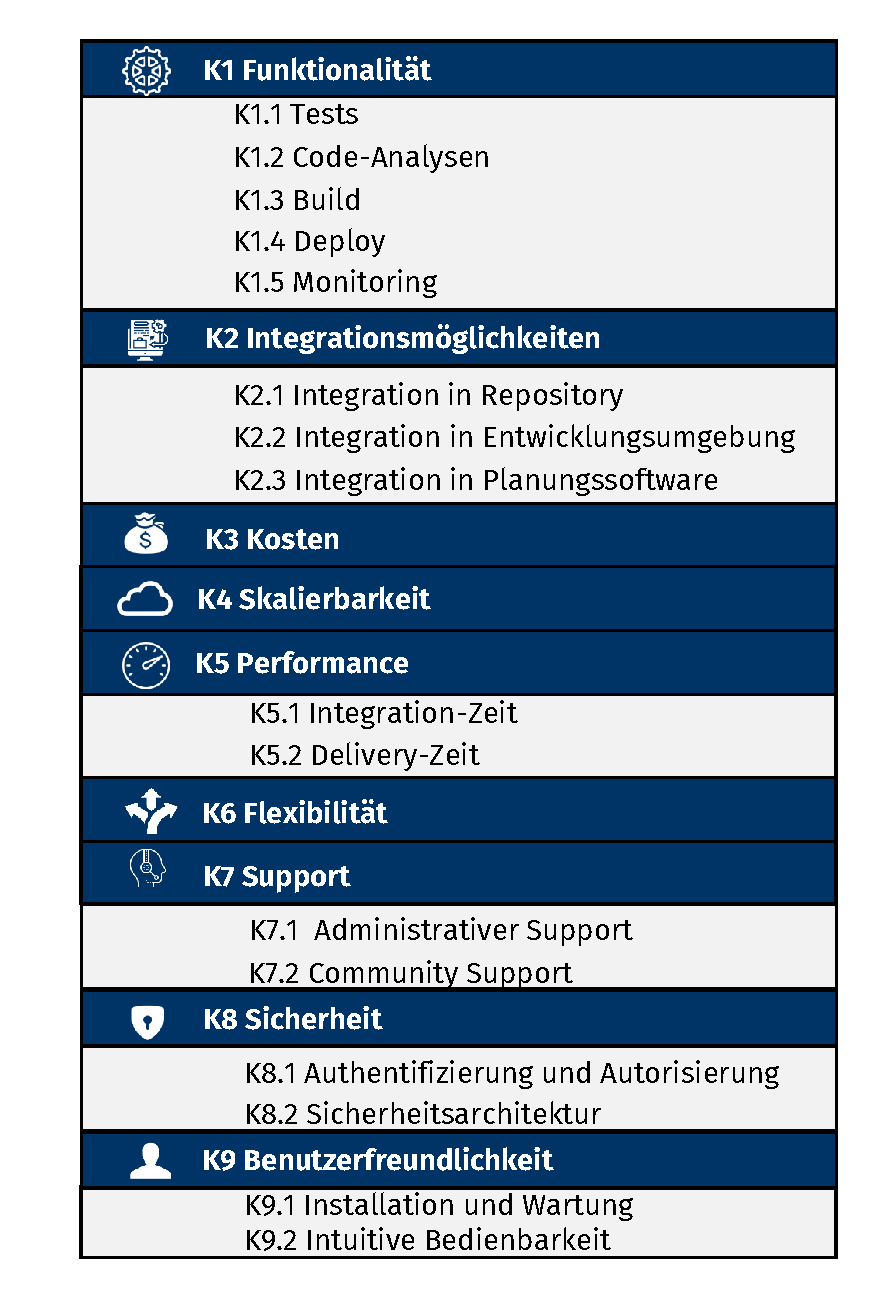
\includegraphics{AHP_B}}
		\caption[Exemplarische Darstellung der Paarvergleichsmatrix im AHP]{Exemplarische Darstellung der Paarvergleichsmatrix im AHP.\\ Eigene Darstellung.}
		\label{fig:AHP_B}
	\end{figure}
\end{center}
\vspace*{-10mm}
So wird dem in Abb. \ref*{fig:AHP_B} exemplarisch dargestellten Kriterium K1 eine wesentlichere Bedeutung als K2 zugeschrieben. Das korrespondieren Äquivalent auf der rechten Matrixhälfte besitzt entsprechend eine Gewichtung von null (\textit{weniger wichtig}). Um der in der Paarvergleichsmatrix getroffenen Gegenüberstellung eine höhere Aussagekraft zu verleihen, müssen die relativen Gewichtungen in prozentuale Werte transformiert werden. Im ersten Schritt müssen hierfür alle Paarvergleichswerte eines Entscheidungskriteriums aufsummiert werden:\\
 \vspace{-6mm}
 \begin{center}
	$V_{k1}$ = $X_{11}+X_{12}+X_{13}$	
 \end{center}
Anschließend muss diese Summe standardisiert werden. Hierfür wird die Gewichtungssumme ($V_{ki}$) eines Kriteriums durch die Gesamtanzahl der in einer Paarvergleichsmatrix (\textit{W}) vergebenen Punkte dividiert. Diese ergibt sich durch eine Betrachtung der in einer Matrix durchgeführten Paarvergleiche. Beinhaltet eine Matrix z.B. drei Kriterien, werden insgesamt 6 Vergleiche durchgeführt. Da für jeden Paarvergleich stets 2 Punkte vergeben werden, entspricht die Gesamtanzahl der Gewichtungspunkte (\textit{W}) bei einer Gegenüberstellung von drei Kriterien zwölf (\textit{12 = 2$\cdot$6}). Anschließend kann die prozentuale Gewichtung eines Entscheidungskriteriums wie folgt berechnet werden:
 \vspace{-8mm}
 \begin{center}
	$W_{k1}$ = $\frac{V_{k1}}{W}$	
 \end{center}
Diese lokale Gewichtung wird für jede Hierarchieebene durchgeführt. Um die globale Gewichtung zu ermitteln wird die Gewichtung jedes Subkriteriums mit den Gewichtungen der übergeordneten Kriterien  multipliziert (s. Abb. \ref*{fig:AHP_B}). Entsprechend dem Gesetz der \textit{totalen Wahrscheinlichkeit} ergeben alle globalen Gewichtungen der AHP-Baum-Blätter die Summe eins. 
In der Literatur wird vorgesehen, dass auf unterster Hierarchieebene ebenfalls eine Gewichtung der Entscheidungskriterien vorgenommen wird \cite[86]{Saaty.2008}. Da dies insbesondere bei auf subjektiven Präferenzen basierenden Problemstellungen eine wichtige Rolle spielt, wird hierbei von dem Leitfaden nach Saaty abgewichen. Stattdessen wird für jedes Kriterium auf unterster Ebene eine feste Metrik definiert, anhand welcher die Alternativen bewertet werden. Letztlich werden die hierbei getroffenen Bewertungen mit den globalen Gewichtungsfaktoren multipliziert und alle Teilbewertungen zu einer gewichteten Gesamtbenotung zusammengezogen. Die Entscheidungsalternative mit der höchsten Gesamtbewertung gilt dabei als optimale Alternative. 
\begin{center}
	\begin{figure}[H]
		\centering
		\scalebox{0.3}{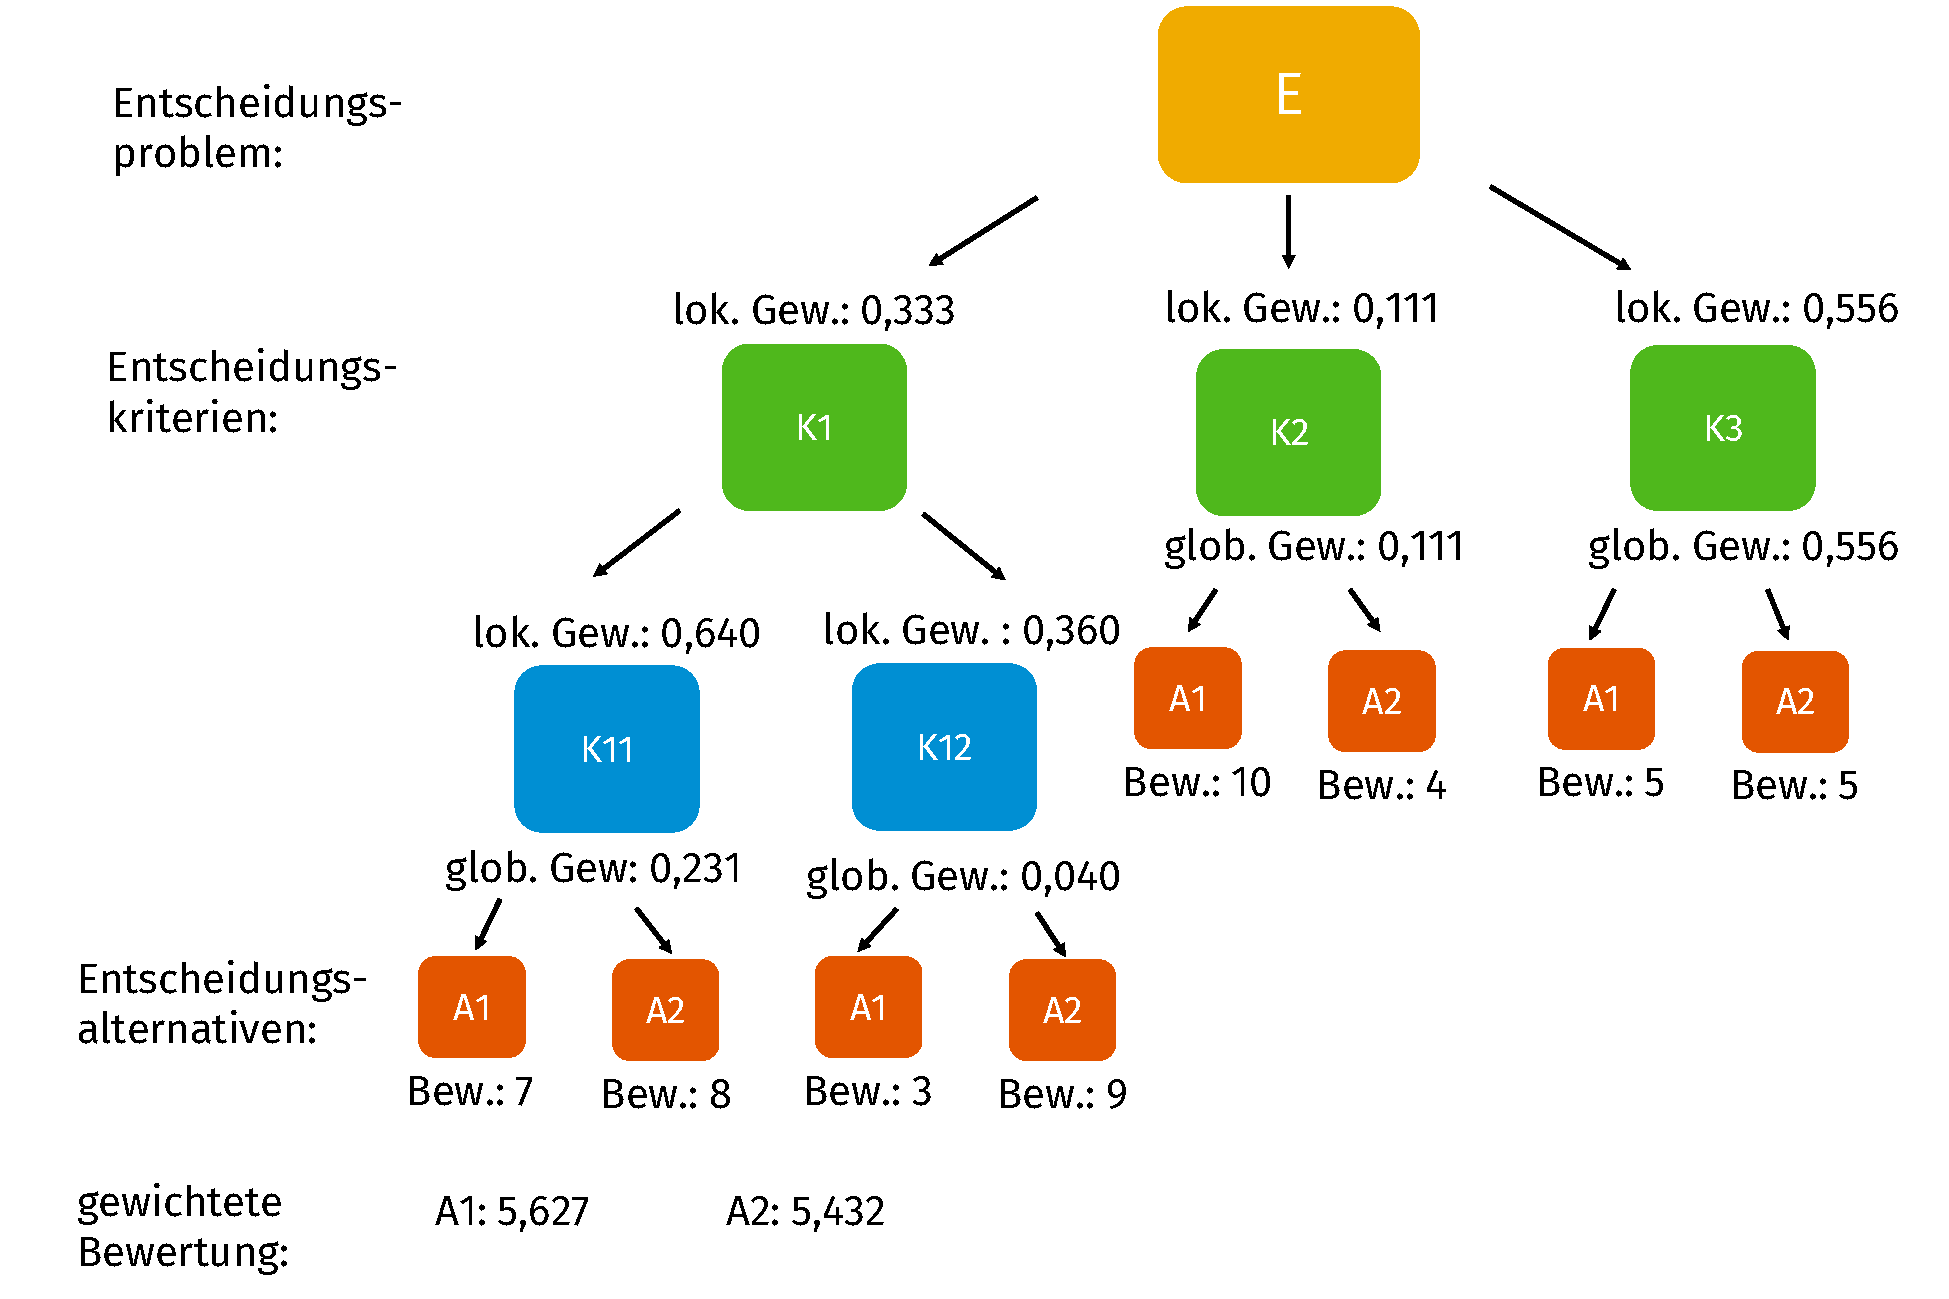
\includegraphics{AHP_H}}
		\caption[Exemplarische Darstellung der hierarchischen Entscheidungsstruktur im AHP]{Exemplarische Darstellung der hierarchischen Entscheidungsstruktur im AHP. Eigene Darstellung.}
		\label{fig:AHP_B}
	\end{figure}
\end{center}
\vspace*{-10mm}